%%%%%% bibliography
%%%% upload WinterSchool2020.bib

\documentclass[11pt]{article}

\usepackage{apacite} %bib style

\usepackage{longtable} 

\usepackage{adjustbox} 

\title{My first replicable Paper}
\author{
        MyFirstName MyLastName\\
        Evans School of Public Policy and Governance\\
        University of Washington\\
        Seattle, WA 98115, \underline{United States}\\
        \texttt{greatguy@uw.edu}
}
\date{\today}



\usepackage{Sweave}
\begin{document}
\Sconcordance{concordance:PaperInR_8.tex:PaperInR_8.Rnw:%
1 23 1 1 0 29 1 1 5 1 1 1 8 6 1 1 8 29 0 1 2 8 1 1 9 4 1 2 2 12 1 1 8 %
14 0 1 2 2 1 1 8 4 1 2 2 15 1 1 5 3 1 2 2 12 1 1 5 4 1 2 2 13 1 1 2 4 0 %
1 2 2 1 1 2 4 0 1 2 3 1 1 2 40 0 1 2 19 1}


\maketitle 

\begin{abstract}
This is an example on how to make a reproducible paper. We are using R from Rstudio, creating an RSweave document. This is a nice start to create a nice paper and get an A+. The next sections will show the steps taken.
\end{abstract}


\section{Introduction}\label{intro}  

This is my intro to my great paper, I will explain the cool things I can do with my new `computational thinking' powers combined with some Latex. This is my intro to my great paper, I will explain the cool things I can do with my new `computational thinking' powers combined with some Latex. This is my intro to my great paper, I will explain the cool things I can do with my new `computational thinking' powers combined with some Latex. This is my intro to my great paper, I will explain the cool things I can do with my new `computational thinking' powers combined with some Latex.


This is my nice intro to my great paper, 
I will explain the cool things 
I can do with my new `computational thinking' 
powers
combined with some Latex.


\section{Exploring Data}\label{explo}


Sections may use a label\footnote{In fact, you can have a label wherever you think a future reference to that content might be needed.}. This label is needed for referencing. For example the next section has label \emph{datas}, so you can reference it by writing: As we see in section \ref{catexplo}.







\subsection{Exploring Categorical Data}\label{catexplo}

Here, I continue doing this nice work, I hope you like it and read it. It has been a very hard work.Here, I continue doing this nice work, I hope you like it and read it. It has been a very hard work.Here, I continue doing this nice work, I hope you like it and read it. It has been a very hard work.Here, I continue doing this nice work, I hope you like it and read it. It has been a very hard work.Here, I continue doing this nice work, I hope you like it and read it. It has been a very hard work.Here, I continue doing this nice work, I hope you like it and read it. It has been a very hard work.

You can see the statistics of categorical variables in Table \ref{catexplore_table}.

% latex table generated in R 3.6.2 by xtable 1.8-4 package
% Fri Feb  7 15:46:31 2020
\begingroup\normalsize
\begin{longtable}{llrrr}
\caption{Freq Table} \\ 
 \textbf{Variable} & \textbf{Levels} & $\mathbf{n}$ & $\mathbf{\%}$ & $\mathbf{\sum \%}$ \\ 
  \hline
Region & Africa & 55 & 27.1 & 27.1 \\ 
   & Asia & 45 & 22.2 & 49.3 \\ 
   & Eurasia & 6 & 3.0 & 52.2 \\ 
   & Europe & 45 & 22.2 & 74.4 \\ 
   & NAmerica & 26 & 12.8 & 87.2 \\ 
   & Oceania & 14 & 6.9 & 94.1 \\ 
   & SAmerica & 12 & 5.9 & 100.0 \\ 
   \hline
 & all & 203 & 100.0 &  \\ 
   \hline
\hline
ONIpolitical & nd & 2 & 2.6 & 2.6 \\ 
   & per & 8 & 10.5 & 13.2 \\ 
   & sub & 4 & 5.3 & 18.4 \\ 
   & sel & 21 & 27.6 & 46.0 \\ 
   & ne & 41 & 54.0 & 100.0 \\ 
   \hline
 & all & 76 & 100.0 &  \\ 
   \hline
\hline
\hline
\label{catexplore_table}
\end{longtable}
\endgroup




%%%%%%

You can see this variable plotted in Figure \ref{catexplore_plot}



\begin{figure}[h]
\centering
\begin{adjustbox}{width=7cm,height=5cm}
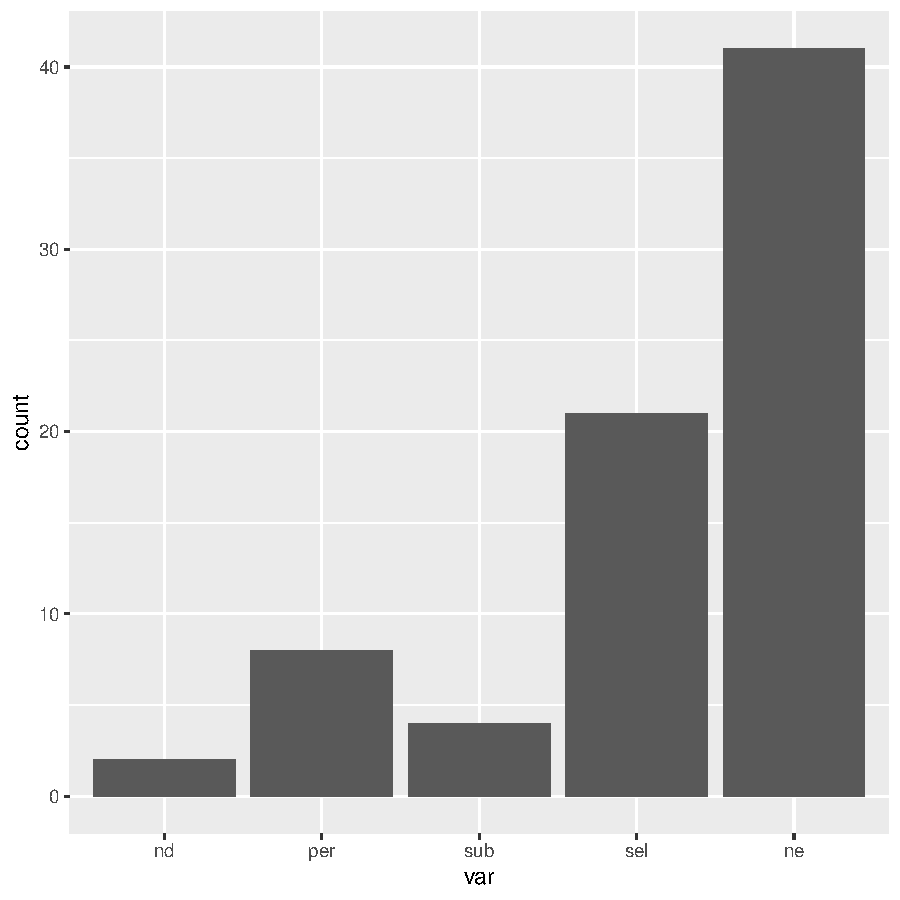
\includegraphics{PaperInR_8-cat_plot}
\end{adjustbox}
\caption{ONI barplot}  %title
\label{catexplore_plot} % for \ref{}
\end{figure}





\subsection{Exploring Numerical Data}\label{numexplo}

Here, I continue doing this nice work, I hope you like it and read it. It has been a very hard work.Here, I continue doing this nice work, I hope you like it and read it. It has been a very hard work.Here, I continue doing this nice work, I hope you like it and read it. It has been a very hard work.Here, I continue doing this nice work, I hope you like it and read it. It has been a very hard work.Here, I continue doing this nice work, I hope you like it and read it. It has been a very hard work.Here, I continue doing this nice work, I hope you like it and read it. It has been a very hard work.Here, I continue doing this nice work, I hope you like it and read it. It has been a very hard work.Here, I continue doing this nice work, I hope you like it and read it. It has been a very hard work.Here, I continue doing this nice work, I hope you like it and read it. It has been a very hard work.

% Table created by stargazer v.5.2.2 by Marek Hlavac, Harvard University. E-mail: hlavac at fas.harvard.edu
% Date and time: Fri, Feb 07, 2020 - 15:46:32
\begin{table}[!htbp] \centering 
  \caption{Stat summary for nummeric vars} 
  \label{numexplore_table} 
\footnotesize 
\begin{tabular}{@{\extracolsep{5pt}}lccccccc} 
\\[-1.8ex]\hline 
\hline \\[-1.8ex] 
Statistic & \multicolumn{1}{c}{Median} & \multicolumn{1}{c}{Mean} & \multicolumn{1}{c}{Min} & \multicolumn{1}{c}{Max} & \multicolumn{1}{c}{Pctl(25)} & \multicolumn{1}{c}{Pctl(75)} & \multicolumn{1}{c}{St. Dev.} \\ 
\hline \\[-1.8ex] 
FHF & 49.00 & 47.24 & 10.00 & 97.00 & 25.25 & 63.00 & 23.72 \\ 
RWB & 28.72 & 32.40 & 6.38 & 84.83 & 23.60 & 38.50 & 16.64 \\ 
\hline \\[-1.8ex] 
\end{tabular} 
\end{table} 
In the Table \ref{numexplore_table}, you realize that the mean of FHF is {\bf47.2424242424242}.



\begin{figure}[h]
\centering
\begin{adjustbox}{width=7cm,height=5.5cm,clip,trim=0cm 0.5cm 0cm 0cm} 
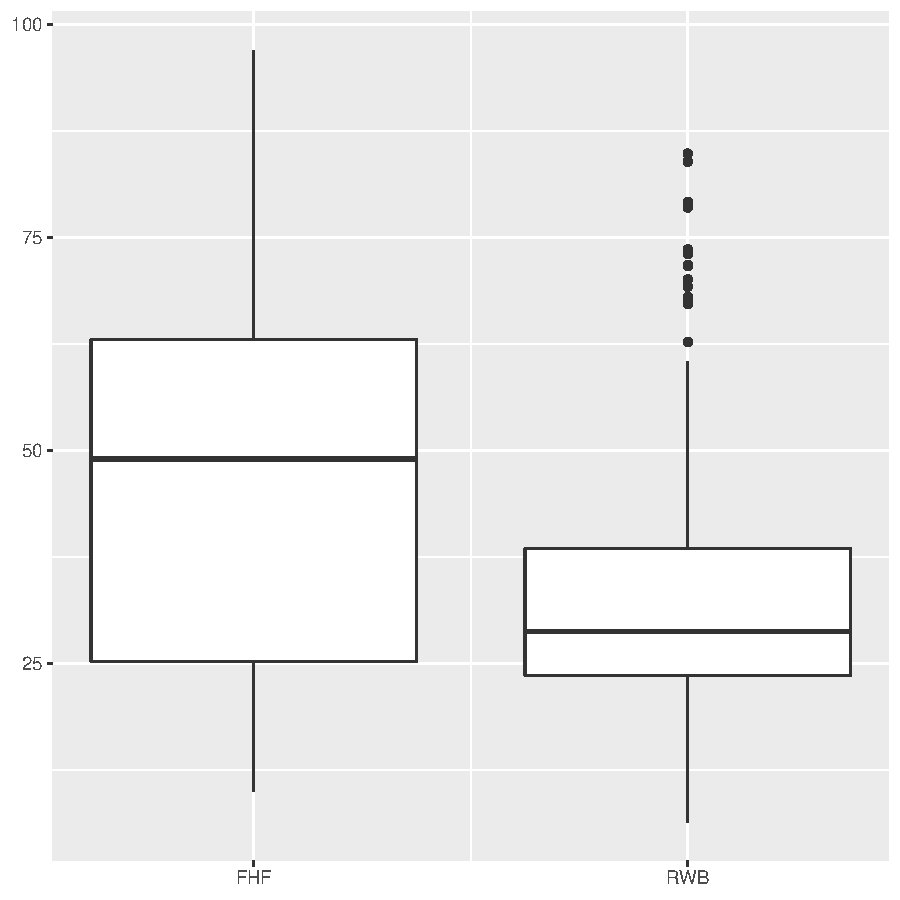
\includegraphics{PaperInR_8-num_plot}
\end{adjustbox}
\caption{boxplots}  
\label{num_plot} 
\end{figure}

%%%%% adding citation
Boxplots were introduced by Tuckey \cite{tukey_exploratory_1977}.

\section{Looking for Relationships}\label{bivar}


Here, I continue doing this nice work, I hope you like it and read it. It has been a very hard work.Here, I continue doing this nice work, I hope you like it and read it. It has been a very hard work.Here, I continue doing this nice work, I hope you like it and read it. It has been a very hard work.Here, I continue doing this nice work, I hope you like it and read it. It has been a very hard work.Here, I continue doing this nice work, I hope you like it and read it. It has been a very hard work.Here, I continue doing this nice work, I hope you like it and read it. It has been a very hard work.Here, I continue doing this nice work, I hope you like it and read it. It has been a very hard work.Here, I continue doing this nice work, I hope you like it and read it. It has been a very hard work.Here, I continue doing this nice work, I hope you like it and read it. It has been a very hard work.

\subsection{Numerical and  Categorical}\label{binumcat}



\begin{figure}[h]
\centering
\begin{adjustbox}{width=7cm,height=7cm} 
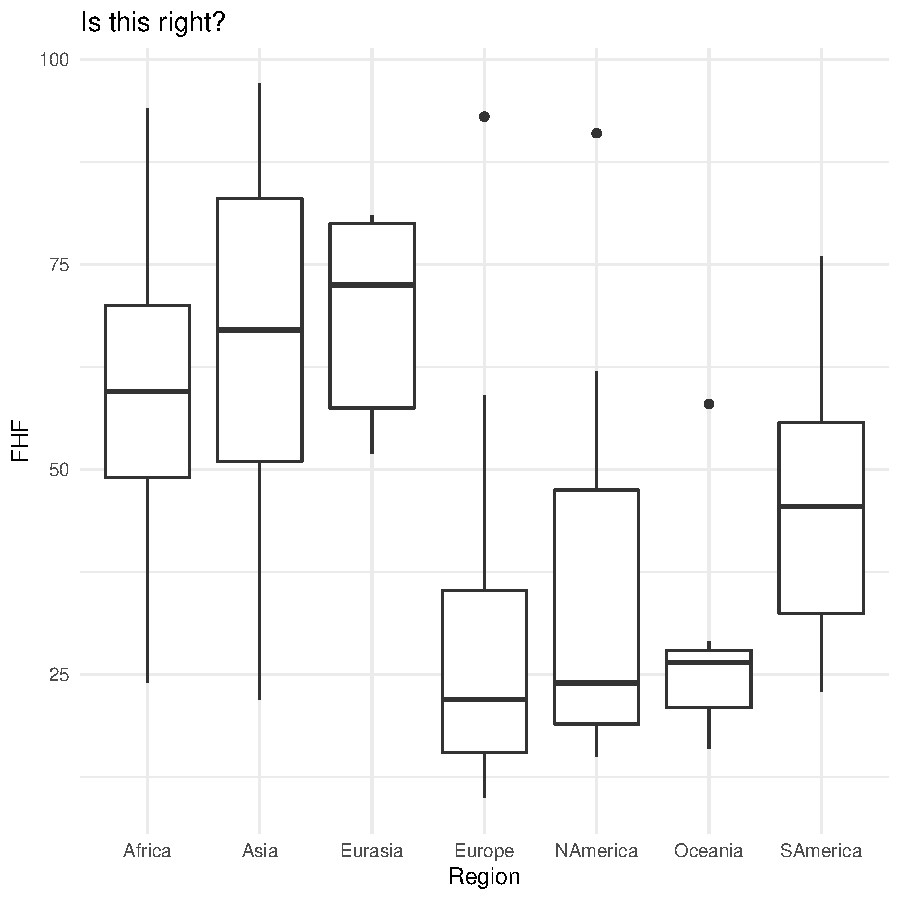
\includegraphics{PaperInR_8-numcat_plot}
\end{adjustbox}
\caption{Boxplots: one numerical by a category.}  
\label{numcat_plot} 
\end{figure}


Here, I continue doing this nice work, I hope you like it and read it. It has been a very hard work.Here, I continue doing this nice work, I hope you like it and read it. It has been a very hard work.Here, I continue doing this nice work, I hope you like it and read it. It has been a very hard work.Here, I continue doing this nice work, I hope you like it and read it. It has been a very hard work.Here, I continue doing this nice work, I hope you like it and read it. It has been a very hard work.Here, I continue doing this nice work, I hope you like it and read it. It has been a very hard work.Here, I continue doing this nice work, I hope you like it and read it. It has been a very hard work.Here, I continue doing this nice work, I hope you like it and read it. It has been a very hard work.Here, I continue doing this nice work, I hope you like it and read it. It has been a very hard work.

\subsection{Numerical and Numerical}\label{binumnum}

Here, I continue doing this nice work, I hope you like it and read it. It has been a very hard work.Here, I continue doing this nice work, I hope you like it and read it. It has been a very hard work.Here, I continue doing this nice work, I hope you like it and read it. It has been a very hard work.Here, I continue doing this nice work, I hope you like it and read it. It has been a very hard work.Here, I continue doing this nice work, I hope you like it and read it. It has been a very hard work.Here, I continue doing this nice work, I hope you like it and read it. It has been a very hard work.Here, I continue doing this nice work, I hope you like it and read it. It has been a very hard work.Here, I continue doing this nice work, I hope you like it and read it. It has been a very hard work.Here, I continue doing this nice work, I hope you like it and read it. It has been a very hard work.




\begin{figure}[h]
\centering
\begin{adjustbox}{width=7cm,height=5.5cm}
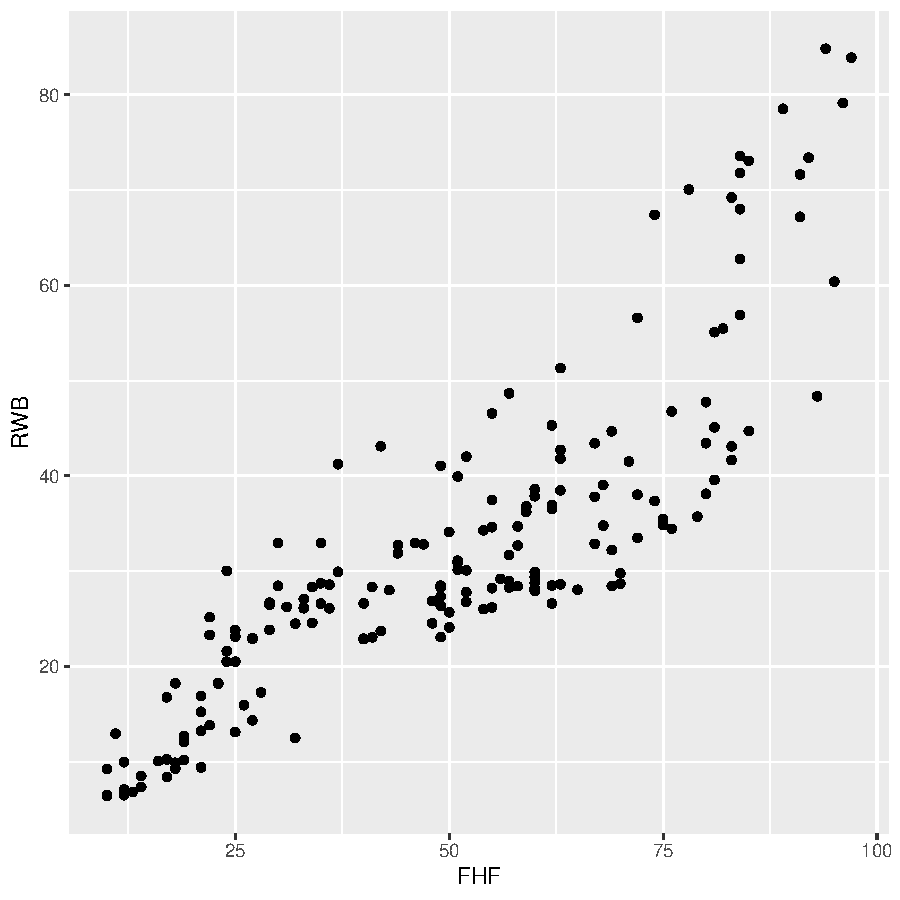
\includegraphics{PaperInR_8-numnum_plot}
\end{adjustbox}
\caption{scatter}  
\label{numnum_plot} 
\end{figure}



%%%%% adding citation
The scatter plot is thought to be invented by  John Frederick W. Herschel \cite{friendly_early_2005}

\section{My Regression}\label{regre}

This is a Regression in R:

\begin{Schunk}
\begin{Sinput}
> regre1=lm(FHF~RWB,data=dataidx)
\end{Sinput}
\end{Schunk}

This is another:

\begin{Schunk}
\begin{Sinput}
> regre2=lm(FHF~RWB+ONIpolitical,data=dataidx)
\end{Sinput}
\end{Schunk}

\clearpage
These is a better summary, and for both:

% Table created by stargazer v.5.2.2 by Marek Hlavac, Harvard University. E-mail: hlavac at fas.harvard.edu
% Date and time: Fri, Feb 07, 2020 - 15:46:33
\begin{table}[!htbp] \centering 
  \caption{Regression Models} 
  \label{regs} 
\begin{tabular}{@{\extracolsep{5pt}}lcc} 
\\[-1.8ex]\hline 
\hline \\[-1.8ex] 
 & \multicolumn{2}{c}{\textit{Dependent variable:}} \\ 
\cline{2-3} 
\\[-1.8ex] & \multicolumn{2}{c}{FHF} \\ 
\\[-1.8ex] & (1) & (2)\\ 
\hline \\[-1.8ex] 
 RWB & 1.198$^{***}$ & 1.061$^{***}$ \\ 
  & (0.054) & (0.109) \\ 
  & & \\ 
 ONIpolitical.L &  & 2.897 \\ 
  &  & (7.114) \\ 
  & & \\ 
 ONIpolitical.Q &  & $-$11.366$^{*}$ \\ 
  &  & (5.888) \\ 
  & & \\ 
 ONIpolitical.C &  & $-$3.126 \\ 
  &  & (4.239) \\ 
  & & \\ 
 ONIpolitical$\hat{\mkern6mu}$4 &  & 2.910 \\ 
  &  & (5.119) \\ 
  & & \\ 
 Constant & 11.104$^{***}$ & 18.087$^{***}$ \\ 
  & (1.979) & (6.230) \\ 
  & & \\ 
\hline \\[-1.8ex] 
Observations & 178 & 76 \\ 
R$^{2}$ & 0.735 & 0.757 \\ 
Adjusted R$^{2}$ & 0.734 & 0.739 \\ 
Residual Std. Error & 12.049 (df = 176) & 12.146 (df = 70) \\ 
F Statistic & 488.606$^{***}$ (df = 1; 176) & 43.529$^{***}$ (df = 5; 70) \\ 
\hline 
\hline \\[-1.8ex] 
\textit{Note:}  & \multicolumn{2}{r}{$^{*}$p$<$0.1; $^{**}$p$<$0.05; $^{***}$p$<$0.01} \\ 
\end{tabular} 
\end{table} 
I hope you like what you see in the Table \ref{regs}.

%%% if you can't cite correctly, add .bib to the name of the reference{ } and run the document again 

%%% if you want to write a math formula in Latex, google it!
$$ P(x) = \frac{1}{{\sigma \sqrt {2\pi } }}e^{{{ - \left( {x - \mu } \right)^2 } \mathord{\left/ {\vphantom {{ - \left( {x - \mu } \right)^2 } {2\sigma ^2 }}} \right. \kern-\nulldelimiterspace} {2\sigma ^2 }}} $$
% Retreived from http://equplus.net/eqninfo/Equation-258.html

%%% don't use underline(_) on Latex. Will have an error.

%%%%% adding bibliography
\clearpage

%\bibliographystyle{abbrv}
\bibliographystyle{apacite}
%\renewcommand{\refname}{Bibliography}
\bibliography{WinterSchool2020.bib}

\end{document}
